\documentclass[a4,11pt]{article}

\usepackage{exercises}
\usepackage{macros}

\usepackage{graphicx}
\usepackage{ngerman}

\vltitel{Lineare Algebra 2}
\dozent{\small{Christian Haase}}
\assistent{\small{Jan Marten Sevenster}}
\tutoren{\small{%
    Theresa Graeber \\[-1ex] Eva Schinzel}}

\semester{Sommersemester 2023%
  % \raisebox{-10mm}[0pt][0pt]{%
  %   \parbox{0pt}{\includegraphics[width=27mm]{../../2015-ana1-L/Vorlesungsmaterial/ana1QR}}}
}

\begin{document}
\vspace*{-17mm}
{
\kopf
}
% \vspace*{-5mm}
% \enlargethispage*{25mm}

\newcounter{chapter}
% \ueblatt{0}{ bla }
\begin{center} \Large \bfseries Hausaufgabe 0 \end{center}
\bigskip
\bigskip

Wir wollen Internetseiten nach ihrer
"`Wichtigkeit"' sortieren. Weisen Sie jeder Internetseite eine Zahl
zu, die ihre Wichtigkeit symbolisiert. Dabei soll eine Seite um so
wichtiger sein, je mehr wichtige Seiten darauf verlinken
("`Back-Links"').
\bigskip

{\bf Ein erster Versuch.} \ Weise jeder Seite die Zahl ihrer Back-Links
zu. 
\bigskip

{\bf Ein Beispiel.} \ Hier ist eine leicht vereinfachte Darstellung des
Internets. Die Pfeile symbolisieren Links.
\begin{center}
  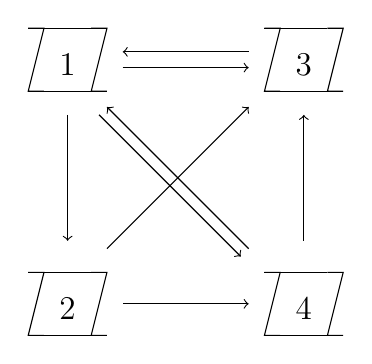
\begin{tikzpicture}[y=-1cm]

% objects at depth 50:
\draw[black] (2.5,5.6) -- (3.3,5.6);
\draw[black] (2.7,6.4) -- (3.5,6.4);
\draw[black] (2.5,5.6) -- (2.7,5.6) -- (2.5,6.4) -- (2.7,6.4);
\draw[black] (3.3,5.6) -- (3.5,5.6) -- (3.3,6.4) -- (3.5,6.4);
\draw[black] (5.5,5.6) -- (6.3,5.6);
\draw[black] (5.7,6.4) -- (6.5,6.4);
\draw[black] (5.5,5.6) -- (5.7,5.6) -- (5.5,6.4) -- (5.7,6.4);
\draw[black] (6.3,5.6) -- (6.5,5.6) -- (6.3,6.4) -- (6.5,6.4);
\draw[black] (5.5,2.5) -- (6.3,2.5);
\draw[black] (5.7,3.3) -- (6.5,3.3);
\draw[black] (5.5,2.5) -- (5.7,2.5) -- (5.5,3.3) -- (5.7,3.3);
\draw[black] (6.3,2.5) -- (6.5,2.5) -- (6.3,3.3) -- (6.5,3.3);
\draw[black] (2.5,2.5) -- (3.3,2.5);
\draw[black] (2.7,3.3) -- (3.5,3.3);
\draw[black] (2.5,2.5) -- (2.7,2.5) -- (2.5,3.3) -- (2.7,3.3);
\draw[black] (3.3,2.5) -- (3.5,2.5) -- (3.3,3.3) -- (3.5,3.3);
\draw[arrows=-to,black] (3.5,5.3) -- (5.3,3.5);
\draw[arrows=-to,black] (5.3,2.8) -- (3.7,2.8);
\draw[arrows=to-,black] (5.3,6) -- (3.7,6);
\draw[arrows=-to,black] (5.3,5.3) -- (3.5,3.5);
\draw[arrows=-to,black] (3.7,3) -- (5.3,3);
\draw[arrows=-to,black] (3,3.6) -- (3,5.2);
\draw[arrows=to-,black] (6,3.6) -- (6,5.2);
\draw[arrows=-to,black] (3.4,3.6) -- (5.2,5.4);
\path (3,3.1) node[text=black,anchor=base] {\large{}$1$};
\path (6,6.2) node[text=black,anchor=base] {\large{}$4$};
\path (6,3.1) node[text=black,anchor=base] {\large{}$3$};
\path (3,6.2) node[text=black,anchor=base] {\large{}$2$};

\end{tikzpicture}%


  "`Das Internet"'
\end{center}
Unser erster Versuch w\"urde Seite 1 die Wichtigkeit $W_1=2$ zuordnen,
Seite 2 Wichtigkeit $W_2=1$, Seite 3 Wichtigkeit $W_3=3$ und Seite 4
Wichtigkeit $W_4=2$.

Dieser Ansatz missachtet die Forderung, dass Links von wichtigeren
Seiten mehr z\"ahlen sollen. So haben Seiten 1 und 4 die gleiche
Wichtigkeit, jedoch ist Seite 1 von der wichtigeren (?) Seite 3
verlinkt, w\"ahrend Seite 4 nur einen Link von der unwichtigen (?)
Seite 2 bekommt.

Dar\"uberhinaus ist der Ansatz nicht sehr demokratisch. Bei der
Bestimmung der Wichtigkeit hat Seite 1 drei Stimmen, w\"ahrend Seite 3
nur eine Stimme hat. Eigentlich sollte Seite 1 nur jeweils ein Drittel
seiner Wichtigkeit \"uber jeden der drei Links verschicken d\"urfen,
Seite 2 m\"usste die Wichtigkeit 50-50 aufteilen, etc.
\bigskip


% moegliche "`Aspekte"':
% Lineare Gleichungssysteme; Existenz/Eindeutigkeit
% Spaltenstochastische Matrizen
% Iterationsverfahren
% Konvergenz
% Matlab Aspekte
% Groesse/Struktur des Webgraphen
% Modifikationen, was macht Google wirklich?
% Wie kann man Google austricksen?

\begin{aufgabe}
  \mbox{}  
  \begin{itemize}  
  \item Installieren Sie \href{www.sagemath.org}{SageMath} auf einem
    Computer, zu dem Sie regelm"a"sig Zugang haben oder erstellen Sie
    sich ein \href{cocalc.com}{CoCalc}-Konto, um SageMath im Browser
    zu benutzen.
  \item Erstellen Sie ein Jupyter Notebook oder eine Sage Worksheet
    und schreiben Sie
\begin{verbatim}
  x=1
  for k in range(2,10):
      x=x+k
  x
\end{verbatim}
    anschlie"send lassen Sie das Programm mit \url{<shift><return>}
    laufen.
    Was tut dieses Programm? 
    Versuchen Sie, die einzelnen Befehle und den Algorithmus zu verstehen.
  \item
    Versuchen Sie, das Programm so abzu\"andern, dass ...
    \begin{itemize}
      \setlength{\itemsep}{0mm}
    \item ... alle nat\"urlichen Zahlen von 1 bis 10 addiert werden.
    \item ... alle nat\"urlichen Zahlen von 1 bis 10 multipliziert werden.
    \end{itemize}
  \end{itemize}
\end{aufgabe}

\begin{aufgabe}
  \mbox{}
  \begin{itemize}
  \item Im Whiteboard
    finden Sie die Datei \ \url{bsp1.sagews}~. % \ sowie \ \url{methode1&2.sagews}~.
    Rufen Sie das "`Programm"' \ \url{methode1} mit den im Abschnitt
    \url{#} \url{Beispiel} \url{1} gesetzten Variablen \url{A}, \url{v} und
    \url{n} auf.
    
    Spielen Sie mit den Parametern \ \url{v, n} \ und beobachten Sie,
    was passiert.
  \item Erkl\"aren Sie, was das mit unserem urspr\"unglichen
    Internet-Problem zu tun hat.

    Hinweis: die Eingabe in \ \url{Beispiel} \url{1} \ entstand aus
    dem "`Internet"' im obigen Beispiel. K\"onnen Sie ein "`Internet"'
    zeichnen, aus dem Eingabe \ \url{Beispiel} \url{2} \ resultiert?
  \item Wie und warum funktioniert es? Funktioniert es immer? Was hei"st
    "`es funktioniert"'?
  \end{itemize}

\end{aufgabe}

\end{document}

%%% Local Variables: 
%%% mode: latex
%%% TeX-master: t
%%% End: 
